\documentclass[logo,reportComp]{thesis}
\usepackage[cpp,pseudo]{mypackage}

\title{操作系统原理实验报告}
\subtitle{实验一:接管裸机的控制权}
\school{数据科学与计算机学院}
\author{陈鸿峥}
\classname{17大数据与人工智能}
\stunum{17341015}
\headercontext{操作系统原理实验报告}
\authorremark{本实验报告用\LaTeX撰写,创建时间:\builddate\today}


\begin{document}

\maketitle

\section{实验目的}
\begin{itemize}
	\item 搭建好操作系统的实验环境,安装虚拟机,生成虚拟软盘
	\item 编写简单的汇编程序接管裸机的控制权,并添加其他显示特性
	\item 将汇编程序放入虚拟软盘中,引导虚拟机启动
\end{itemize}

\section{实验要求}
% 实验目的和实验要求由老师提供实验项目文档中获取
\begin{enumerate}
	\item 搭建和应用实验环境:虚拟机安装,生成一个基本配置的虚拟机XXXPC和多个1.44MB容量的虚拟软盘。
	\begin{itemize}
		\item 将其中一个虚拟软盘用DOS格式化为DOS引导盘
		\item 用WinHex工具将其中一个虚拟软盘的首扇区填满你的个人信息
	\end{itemize}
	\item 接管裸机的控制权:设计XXXPC的一个引导扇区程序,将字符`A'从屏幕左边某行位置45度角下斜射出,保持一个可观察的适当速度直线运动,碰到屏幕的边后产生反射,改变方向运动,如此类推,不断运动。
	将这个程序的机器码放进放进第三张虚拟软盘的首扇区,并用此软盘引导你的XXXPC,直到成功。
	\begin{itemize}
		\item 在此基础上,增加你的个性扩展,如同时控制两个运动的轨迹,或炫酷动态变色,个性画面等,自由不限。
		\item 在屏幕某个区域特别的方式显示你的学号姓名等个人信息。
	\end{itemize}
\end{enumerate}

\section{实验方案}
% 包括:硬件或虚拟机配置方法、软件工具与作用、方案的思想、相关原理、程序流程、算法和数据结构、程序关键模块,结合代码与程序中的位置位置进行解释。不得抄袭,否则按作弊处理。
% 实验方案包括相关基础原理、实验工具和环境、程序流程和算法思想、数据结构与程序模块功能说明,代码文档组成说明等
\subsection{实验环境}
\begin{itemize}
	\item Windows 10系统 + Ubuntu 18.04(LTS)子系统\\
	Windows系统下有图形界面,使用虚拟机比较简单;而Linux系统对于各种编译环境等的设置、调试都会比较简单,因而这里采用了\textbf{子系统}的方法,这是近两年微软才提供的一种非常新颖的方法,在微软应用商店即可下载。
	注意子系统并非双系统,子系统可以直接访问原系统内的文件,无需挂载硬盘,而且对于原始系统的占用非常少!
	\item gcc 7.3.0 + nasm 2.13.02 + gdb\\
	这些是本机的编译环境,gcc用于编译C/C++程序,而nasm则用于编译汇编程序,gdb用于在Linux环境下调试程序。
	\item Oracle VM VirtualBox 5.2.8\\
	这里采用了Oracle的VirtualBox,一方面是之前已经安装,另一方面则是比较轻量,而且基本虚拟机的操作都可支持。
	\item Sublime Text 3\\
	文本编辑器,编写程序利器,除去常见的文本操作、代码高亮等,还可以添加大量插件,也直接查看二进制文件并进行修改。
\end{itemize}

\subsection{虚拟机配置方法}
\begin{enumerate}
	\item 打开VirtualBox,点新建,输入名称(这里用我的名字命名,即\verb'CHZPC'),(操作系统)类型Other,版本Other/Unknown
	\item 内存大小设最小4M即可
	\item 不添加虚拟硬盘,然后创建
	\item 在创建的\verb'CHZPC'的菜单中点设置-存储-添加软盘控制器
	\item 在``控制器:Floppy''后面点添加虚拟软驱
	\item 添加之后构造好的虚拟软盘``img''文件,如图\ref{fig:floppy_disk}所示
\begin{figure}[H]
\centering
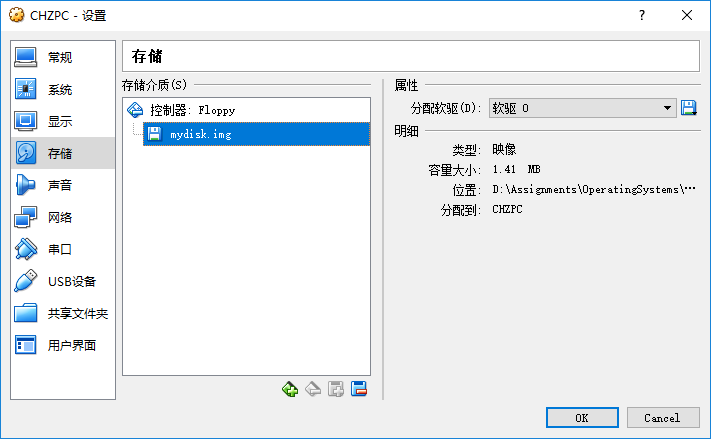
\includegraphics[width=0.6\linewidth]{fig/floppy_disk.PNG}
\caption{添加虚拟软盘}
\label{fig:floppy_disk}
\end{figure}
\end{enumerate}

启动顺序:软驱、光驱、硬盘

\section{实验过程与结果}
% 包括:主要工具安装使用过程及截图结果、程序过程中的操作步骤、测试数据、输入及输出说明、遇到的问题及解决情况、关键功能或操作的截图结果。不得抄袭,否则按作弊处理。
由于VirtualBox已经安装于电脑,故具体安装过程在此不再赘述。

\subsection{搭建和应用实验环境}
\subsubsection{配置虚拟机}
按照``虚拟机配置方法''一节的步骤,可以成功建立名为\verb'CHZPC'的虚拟机,如图\ref{fig:virtual_machine_configuration}所示。
\begin{figure}[H]
\centering
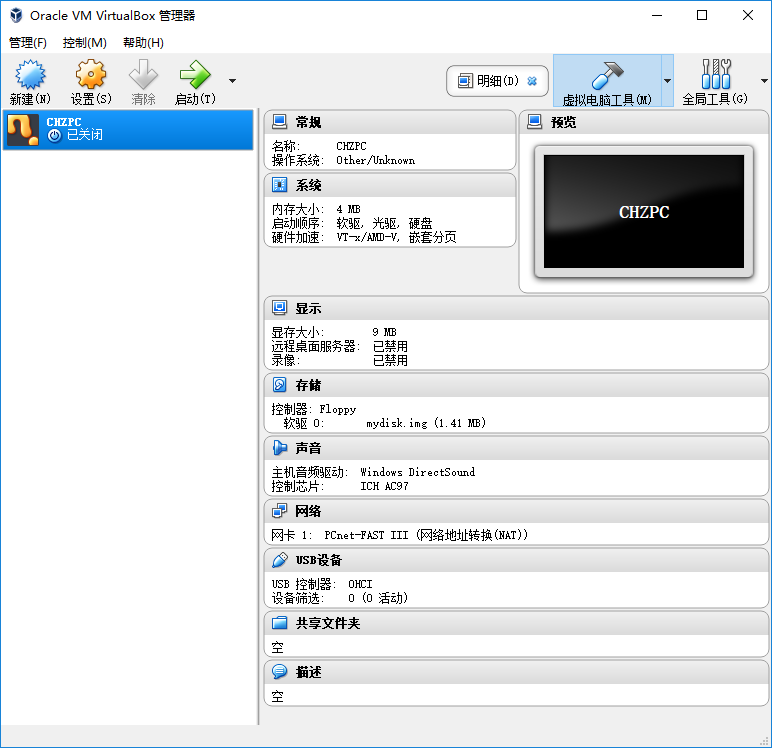
\includegraphics[width=0.6\linewidth]{fig/virtual_machine_configuration.PNG}
\caption{虚拟机具体参数}
\label{fig:virtual_machine_configuration}
\end{figure}

\subsubsection{创建并格式化虚拟软盘}
实际上在Linux系统中,创建一个虚拟软盘十分简单,调用内置的\verb'mkfs'指令即可。
这里我们直接创建一个1.44M的虚拟软盘,注意以前的算法跟现在不一样,1.44M即为1440KB,故输入以下指令
\begin{lstlisting}[language=bash]
/sbin/mkfs.msdos -C mydisk.img 1440
\end{lstlisting}
得到
\begin{figure}[H]
\centering
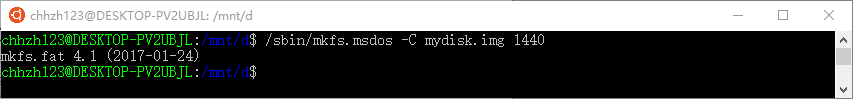
\includegraphics[width=0.8\linewidth]{fig/create_disk.PNG}
\caption{创建虚拟软盘}
\label{fig:create_disk}
\end{figure}

注意图\ref{fig:create_disk}中还显示\verb'mkfs.fat 4.1',代表软盘不仅被创建,还已经被格式化了。
从图\ref{fig:mydisk}中看也确实如此,见32行的\verb'55aa'。

\begin{figure}[H]
\centering
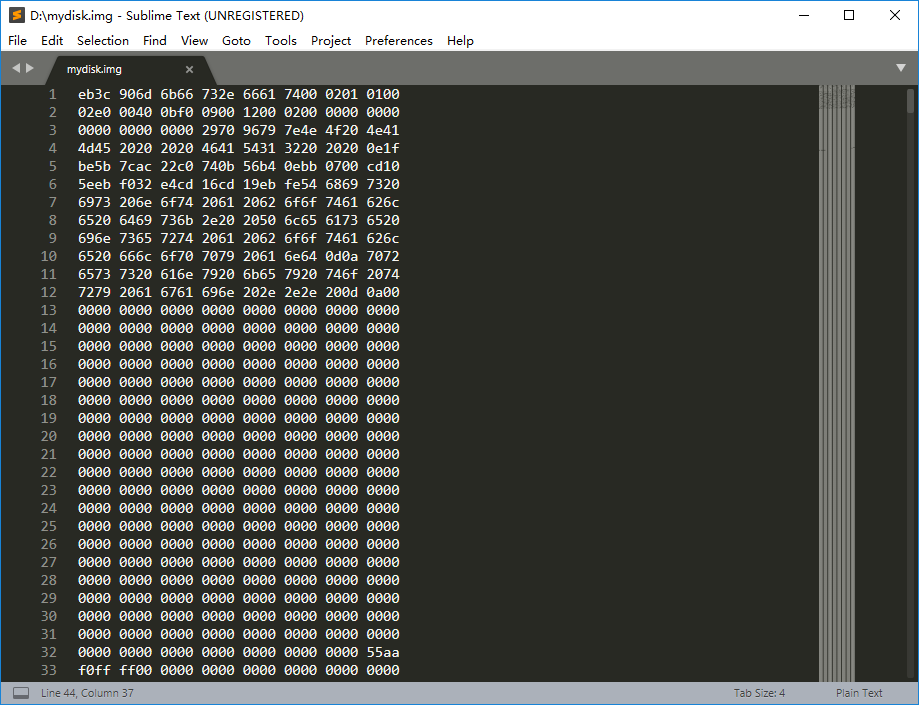
\includegraphics[width=0.8\linewidth]{fig/mydisk.PNG}
\caption{mydisk软盘内容}
\label{fig:mydisk}
\end{figure}

\subsubsection{填满个人信息}
\textbf{这里不采用WinHex的方法,本人自己用Python编写了一个程序},将格式化后的\verb'mydisk.img'虚拟软盘的首扇区填入我的个人信息。
\begin{lstlisting}[language=python]
# fillwords.py
info = "17341015 CHZ"
infob = bytes(info,"ascii")
myname = bytearray(open("mydisk.img","rb").read())
output = open("myname.img","wb")
j = 0
for i in range(513): # fill all
# for i in range(myname.find(b"\xfe")+1,510): # fill part
	myname[i] = ord(info[j])
	j = (j+1) % len(info)
output.write(myname)
\end{lstlisting}

在命令行中直接执行\verb'python fillwords.py'即可。
注意本程序还提供了两种模式:
\begin{itemize}
	\item Fill All模式:将首扇区除最后的\verb'55aa'全部填满信息(见图\ref{fig:fillall}),但是会导致引导盘失效
	\item Fill Part模式:将首扇区除引导部分填满个人信息,这在加载入虚拟机时会正常显示
\end{itemize}
\begin{figure}[H]
\centering
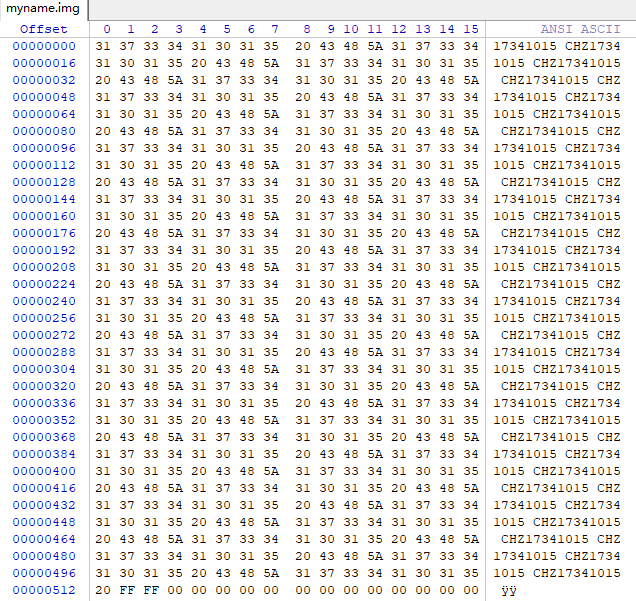
\includegraphics[width=0.8\linewidth]{fig/fillall.PNG}
\caption{Fill All模式}
\label{fig:fillall}
\end{figure}
\begin{figure}[H]
\centering
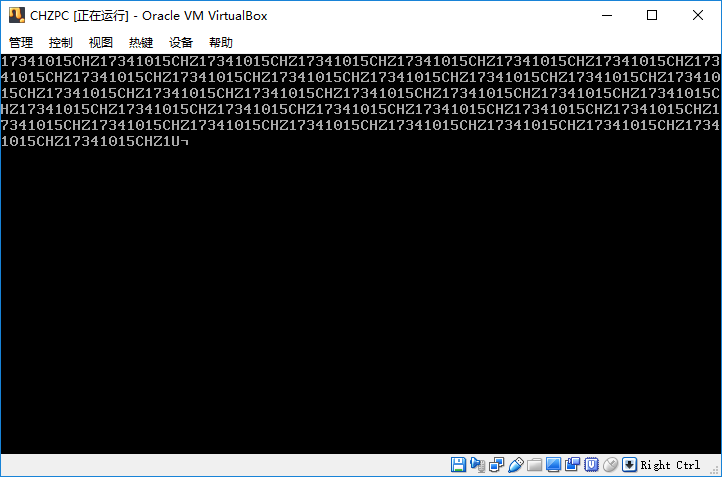
\includegraphics[width=0.8\linewidth]{fig/fillpart.PNG}
\caption{Fill Part模式}
\label{fig:fillpart}
\end{figure}


\subsection{接管裸机控制权}
\subsubsection{编写引导扇区程序}
注意显存的大小为$80\times 25$,故以横向为$x$轴,纵向为$y$轴建立坐标系,原点位于左上角,并且$y$轴正方向向下。
\begin{itemize}
	\item 常量
	\begin{itemize}
		\item 四个方向:右下\verb'Dn_Rt'、右上\verb'Up_Rt'、左上\verb'Dn_Lt'、左下\verb'Dn_Lt'(相当于C/C++语言中的枚举量)
		\item 边界:\verb'MAX_X=80'、\verb'MAX_Y=25'
		\item 延迟变量:\verb'in_delay'、\verb'out_delay'
	\end{itemize}
	\item 数据结构:其他的数据\verb'px1,py1,drt1,char1,color1'等与下面同理
	\begin{itemize}
		\item 字符的坐标:\verb'(px,py)'
		\item 字符运动的方向:\verb'drt'
		\item 字符的内容:\verb'char'
		\item 字符的颜色:\verb'color'
	\end{itemize}
	\item 数据段:用\verb'org 7c00h'指令跳转至对应逻辑地址的位置,进而可以正常使用数据段中的符号访问内存
% 主引导扇区数据为 512 字节,处理器会将主引导扇区的数据加载到逻辑地址 0x0000:0x7c00 中,然后检测最后两字节是否为0x55 和 0xAA, 若存在则主引导扇区有效, 以一个段间转移指令jmp 0x0000:0x7c00 跳到那里继续执行,数据段的位置也要作相应修改。
	\item 字符运动:
	\begin{itemize}
		\item 沿着原来方向,增加一个单位的移动
		\item 如果超出边界,则按照物理规则进行反弹
		\item 这里每一个方向都有两种反弹情况,采用分类讨论的方法,将所有情况枚举了出来,分别考虑
		\item 确定变化规则后,修改\verb'px'和\verb'py'的值
		\item 最后要将新的\verb'px'和\verb'py'的值存回内存
	\end{itemize}
	\item 字符显示
	\begin{itemize}
		\item 为适应人眼,字符变化速度不能过快,故在生成新的字符之前,需要有一个延迟等待(\verb'in_delay'$\times$\verb'out_delay')
		\item 注意文本模式显存段地址\verb'gs'为\verb'B800h',连续两个字节的低位为字符的ASCII码值,高位为字符的显示方式(详情见参考资料,可将低位存于\verb'al',高位存于\verb'ah'中,则显示读取时可直接访问\verb'ax')。
		因而需要计算出要显示字符相对于段地址的偏移量\verb'di',即$(80\times py + px)\times 2$。
		用\verb'mul'指令可以计算出来,根据这个偏移量获得显示字符的地址\verb'[gs:di]'。
		\item 在显示器正中央显示个人信息。
		一开始个人信息以字符串\verb'msg'形式存储于数据段中,通过不断循环读入显示可实现。
	\end{itemize}
	\item 主引导区有效标记:由于采用Linux的\verb'mkfs'和\verb'dd'指令,故不需在汇编程序中考虑,但是需要小心编译出来的二进制文件大小不能大于512B。
	\item 亮点
	\begin{itemize}
		\item 采用\verb'call'和\verb'ret'函数调用的方法,更加容易分开各个模块
		\item 采用宏(macro),使得重复代码只需编写一遍,由编译器负责帮你展开,进而可以方便操控多个字符的运动
		\item 同时控制两个字符(再多的话就超512B了!),并且不断变色
		\item 名字信息用炫酷青色显示在屏幕正中央,与字符交错,且字符移动显示时不会将名字信息清除
	\end{itemize}
\end{itemize}

伪代码程序如下
\begin{algorithm}[H]
\centering
\begin{algorithmic}[1]
\While{\textbf{true}}
\State Call delay
\State Move and show char1
\State Move and show char2
\State Show personal info
\EndWhile
\end{algorithmic}
\caption{Fantastic Words}
\end{algorithm}
具体x86程序见附录\ref{sec:code}程序清单。


\subsubsection{引导PC启动}
将上文编写的\verb'show.asm'用\verb'nasm'进行编译,并生成二进制文件。
\begin{lstlisting}[language=bash]
nasm show.asm -o show.bin
\end{lstlisting}

利用Linux内置的\verb'dd'指令,可以将将编译出来的二进制文件复制到虚拟软盘中。
\begin{lstlisting}[language=bash]
dd if=show.bin of=mydisk.img bs=1440k conv=notrunc
\end{lstlisting}
其中,\verb'bs'指示软盘大小,\verb'conv=notrunc'表示复制时不截断,即不清除超过\verb'show.bin'大小的部分。

\begin{figure}[H]
\centering
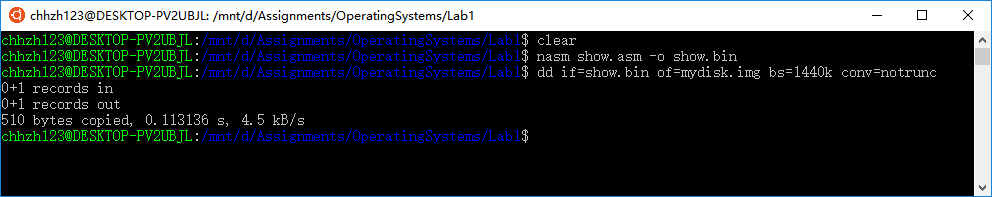
\includegraphics[width=0.8\linewidth]{fig/nasm.PNG}
\caption{编译拷贝过程}
\label{fig:nasm}
\end{figure}
由图\ref{fig:nasm}中可以见到,\verb'show.bin'大小刚好就是510B,没有超过第一个扇区,且最后两位\verb'55aa'也被保留下来。

运行CHZPC,可以得到如图\ref{fig:result}所示的炫酷变色效果。
\begin{figure}[H]
\centering
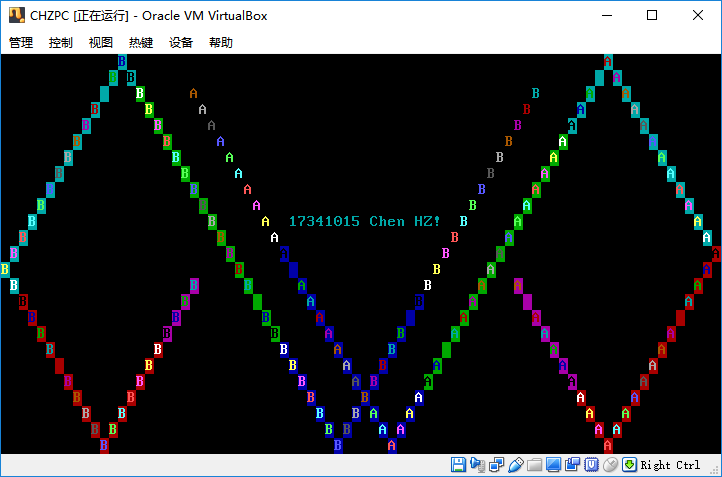
\includegraphics[width=0.8\linewidth]{fig/result.PNG}
\caption{炫酷变色效果}
\label{fig:result}
\end{figure}
在本实验中,中间我的名字以炫酷青色显示,而周围两个字符A和B则从两侧发射,构成一个大V形,然后反弹,同时伴有每格变色功能,相当酷炫!


\section{实验总结}
% 每人必需写一段,文字不少于500字,可以写心得体会、问题讨论与思考、新的设想、感言总结或提出建议等等。不得抄袭,否则按作弊处理。
这次实验虽然是操作系统的第一次实验,但相当折腾,前前后后折腾了我几天时间,查阅了大量网页和资料,才最终将其完成。
下面列出本次实验出现问题的几个点详细阐述。

\begin{enumerate}
\item 由于大多操作系统实验书籍都采用软盘做引导,但是现在早就没有软盘了,所以只能自己虚拟一个出来。
然而说起来轻巧,实际怎么虚拟是需要查阅资料的。
虽然知道Linux环境下应该可以快速虚拟出软盘,但是一开始查到的资料都没有提及虚拟过程,而直接到拷贝\verb'dd'那一步。
中文找不到相关资料,那就用英文搜吧,然而也搜不出来。
查了很久才发现我将软盘的英文的英文搞错了,直觉上想当然就认为是virtual disk,但它的英文是floppy disk,真是有意思!
这回就很快在Stack Overflow搜索到了相关指令,将软盘虚拟了出来。

\item 虚拟出软盘之后第二的难关是修改软盘的数据,在网上下载了WinHex软件,但竟然要收费,免费版本甚至不支持1.44MB软盘的保存。
想着找一些简单的方法,那就搜Linux环境下是否有现成的指令(如\verb'dd'),可以直接用某一字符串填充软盘的。
但搜了很久也没有这样现成的指令。
既然如此一气之下就自己写一个工具去修改吧。
于是便有了前文的Python程序。
但是写这个Python程序也花了不少功夫,主要是对二进制文件的处理上面,\\因为对Python的\verb'bytes'和\verb'bytearray'都不是很熟悉,所以踩了不少坑。
短短几行代码也调试了挺长时间,最终才成功将对应位置的字符修改并写入。

\item 然后就到实际的汇编代码编写。
老师提供的程序根本运行不了,于是便只好逐行读,逐行理解,然后仿照着例子重新编写汇编程序。
尽管上个学期计算机组成原理的课程已经写过汇编程序,但是编程语言只要一段时间不练,很快就会忘了,更何况是汇编这么难懂的语言。
而且此次编写的汇编程序与我之前认知的有一定差异,比如没有显式声明代码段\verb'.code'、数据段\verb'.data'等等。
这可能是因为编译器帮我们补全的缘故。
这里汇编我沿用nasm的语法,但是网上关于nasm的文档很少,关于微软masm语法反而会多些,这也给搜索资料带来了一定的麻烦。

\item 花费好大功夫把汇编程序写完,写了近两百行,却发现死活没法正确读取数据段内的数据/字符串。
希望通过nasm+gdb调试代码,但用尽各种方法总会出现形形色色的问题,要么编译目标机器不对(32位和64位),要么gdb无法加载入调试信息,要么根本没法运行,而这个问题到现在都没有解决。

\item 既然没有办法通过外部调试工具进行调试,那就只能通过人工逐行运行了,这个过程是十分痛苦的。
折腾得死去活来之间,我突然发现\verb'org 7c00h'这条指令被我注释掉了。
查阅了资料才发现这条指令事关数据段的位置,将其注释掉当然也就没法正确访问数据了,进而导致乱码。
因此,重新将该指令添加上即可正常运行。

\item 欢天喜地解决了前面的所有问题,单一字符的程序终于可以正常运行了,然后开始考虑多个字符的情况。
编写完多字符程序编译后,将二进制流拷入软盘,却发现超出了一个扇区的大小。
于是又得重新回到汇编程序中,回炉重造。
绞尽脑汁去缩减代码,将大量冗余的指令删除,最大化利用每一条指令,最后缩减到刚刚好510B也真是奇迹。

\item 修改完程序运行却出现了如图\ref{fig:bug}所示的离奇事件。
A或B两者之一都可以正常运行,而叠加到一起竟然有一个就会出错。
\begin{figure}[H]
\centering
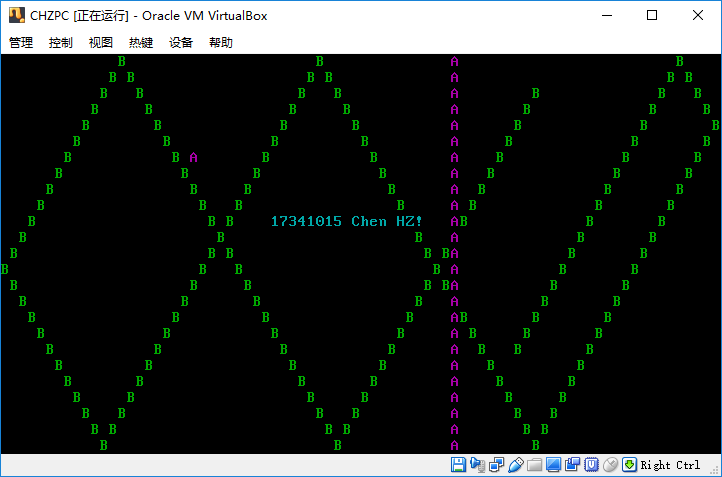
\includegraphics[width=0.8\linewidth]{fig/bug.PNG}
\caption{没有规定读取字符长度的后果}
\label{fig:bug}
\end{figure}
这一个bug虽然离奇,但通过一定的调试,还是可以发现问题所在的。
原因是我将两个字符的坐标数据存在邻近的地方,而在存取数据时我并没有意识到其默认访问大小是\verb'word'(这也与我选择的寄存器有关,因此编译器并没有报错)。
在连续访问中很容易就将后者的数据也修改了造成错误。
因此在汇编编写过程中一定要考虑清楚每个数据的大小,用好特定长度的寄存器,声明好访存的大小(是\verb'byte'还是\verb'word'等)。

\end{enumerate}

最终最终,虚拟机终于能被引导进入程序,并显示出炫酷效果。

总的来说,第一次实验就学到了很多东西。

一方面配置好基本的OS实验环境,学会\verb'dd'、\verb'mkfs'、\verb'nasm'等Linux操作。
学会主引导扇区的工作原理,比如从\verb'7c00h'开始执行;也明白显存的显示机理,用两字节表示一个字符的显示模式,从\verb'B800h'开始地址计数;同时明白怎么编写引导程序使虚拟机能够正常运行。

另一方面则是了解了x86汇编的基本知识,知道有哪些常见指令(包括\verb'mov'、\verb'jmp'、\verb'cmp'、\verb'mul'等),知道这些指令的工作机理,了解x86有哪些寄存器(包括通用寄存器GPR、段寄存器等);知道在nasm语法中怎么使用宏和函数调用让程序变得结构化及简练。

希望在今后的实验中能提高效率,提升码力,更好地完成本学期操作系统的任务吧。

\section{参考资料}
\begin{enumerate}
	\item 李忠,王晓波,余洁,《x86汇编语言-从实模式到保护模式》,电子工业出版社,2013
	\item x86汇编导引,\url{http://www.cs.virginia.edu/~evans/cs216/guides/x86.html#instructions}
	\item x86寄存器,\url{http://www.hep.wisc.edu/~pinghc/x86AssmTutorial.htm}
	\item Linux环境下创建虚拟软盘,\url{https://untitledfinale.wordpress.com/2007/10/09/create-mount-and-copy-floppy-disks-images-under-linux/}
	\item dd命令使用详解,\url{https://www.cnblogs.com/jikexianfeng/p/6103500.html}
	\item 汇编数据类型db,dw,dd,\url{https://stackoverflow.com/questions/10168743/which-variable-size-to-use-db-dw-dd-with-x86-assembly}
\end{enumerate}

\appendix
\appendixconfig
\section{程序清单}
\label{sec:code}
\begin{lstlisting}[language={[x86masm]Assembler}]
; show.asm
; Graphic memory: 25*80 Text Mode

; Constants
Dn_Rt equ 1     ; D-Down, U-Up, R-right, L-Left
Up_Rt equ 2
Up_Lt equ 3
Dn_Lt equ 4
MAX_X equ 80
MAX_Y equ 25
in_delay equ 60000 ; control the speed
out_delay equ 6000  ; outer loop

; Disk Initialization
	org 7c00h               ; ORG (origin) is used to set the assembler location counter
; start:
	mov ax, 0B800h          ; graphic memory start address, ax is GPR
	mov gs, ax              ; GS = B800h segment register

%macro OneChar 5
	; px: position x
	; py: position y
	; drt: direction
	; char: char ascii
	; color
	mov ax, [%1]
	mov [px], ax
	mov ax, [%2]
	mov [py], ax
	mov al, [%3]
	mov [drt], al
	mov al, [%4]
	mov [char], al
	mov al, [%5]
	inc al
	mov [color], al         ; change colors

	call onemove

	;;; Store back to memory ;;;
	mov dx, [px]
	mov [%1], dx
	mov dx, [py]
	mov [%2], dx
	mov dl, [drt]           ; bytes, be careful!
	mov [%3], dl
	mov dl, [color]
	mov [%5], dl
%endmacro

mainloop:
	call delayloop
	OneChar px1,py1,drt1,char1,color1
	OneChar px2,py2,drt2,char2,color2
	call showinfo
	jmp mainloop

showinfo:
	mov esi, msg            ; move msg's address into si (GPR)
	mov di, (10*80+32)*2    ; middle of the 10th line
	mov cx, 17              ; loop index
	infoloop:
		mov bl, byte [esi]
		inc si                  ; next char
		mov bh, 03h             ; property
		mov word [gs:di], bx
		add di, 2               ; 2 Bytes
		loop infoloop           ; automatically minus 1 from cx
	ret

delayloop:
	mov ecx, out_delay
	outloop:
		mov eax, in_delay
		inloop:
			dec eax
			jg inloop
	loop outloop
	ret

onemove:
	cmp byte[drt], 1
	jz DnRt
	cmp byte[drt], 2
	jz UpRt
	cmp byte[drt], 3
	jz UpLt
	cmp byte[drt], 4
	jz DnLt
onemoveret:
	ret

;;;;; Down Right ;;;;;
DnRt:
	inc word[px]
	inc word[py]
	mov ax, word[py]
	cmp ax, MAX_Y            ; px = MAX_Y?
	je dr2ur                 ; jump if the result of the last arithmetic operation was zero
	mov ax, word[px]         ; PX = MAX_X?
	cmp ax, MAX_X
	je dr2dl
	jmp show
dr2ur:
	mov word[py], MAX_Y-2
	mov byte[drt], Up_Rt
	jmp show
dr2dl:
	mov word[px], MAX_X-2
	mov byte[drt], Dn_Lt
	jmp show

;;;;; Up Right ;;;;;
UpRt:
	inc word[px]
	dec word[py]
	mov ax, word[px]
	cmp ax, MAX_X
	je ur2ul
	mov ax, word[py]
	cmp ax, -1
	je ur2dr
	jmp show
ur2ul:
	mov word[px], MAX_X-2
	mov byte[drt], Up_Lt
	jmp show
ur2dr:
	mov word[py], 1
	mov byte[drt], Dn_Rt
	jmp show

;;;;; Up Left ;;;;;
UpLt:
	dec word[px]
	dec word[py]
	mov ax, word[py]
	cmp ax, -1
	je ul2dl
	mov ax, word[px]
	cmp ax, -1
	je ul2ur
	jmp show
ul2dl:
	mov word[py], 1
	mov byte[drt], Dn_Lt
	jmp show
ul2ur:
	mov word[px], 1
	mov byte[drt], Up_Rt
	jmp show

;;;;; Down Left ;;;;;
DnLt:
	dec word[px]
	inc word[py]
	mov ax, word[px]
	cmp ax, -1
	je dl2dr
	mov ax, word[py]
	cmp ax, MAX_Y
	je dl2ul
	jmp show
dl2dr:
	mov word[px], 1
	mov byte[drt], Dn_Rt
	jmp show
dl2ul:
	mov word[py], MAX_Y-2
	mov byte[drt], Up_Lt
	jmp show

;;;;; Show words ;;;;;
show:
	xor ax, ax              ; Compute memory address, ax = 0
	mov ax, word[py]        ; ax = y
	mov bx, 80              ; bx = 80
	mul bx                  ; dstop: ax = 80*y, srcop: parameter (bx)
	add ax, word[px]        ; ax = 80*y + x
	mov bx, 2               ; bx = 2
	mul bx                  ; ax = (80*y + x) * 2
	mov bp, ax              ; bp = ax, position
	mov ah, [color]         ; AH = char property, 0000:Black, 1111:White, high bits
	mov al, byte[char]      ; AL = char value (default 20h=space), low bits
	mov word[gs:bp], ax     ; AX = (AH,AL)
	jmp onemoveret

;;;;; Data Segment ;;;;;
datadef:
	px dw 0
	py dw 0
	drt db Dn_Rt                    ; Down Right
	char db '*'
	color db 00000111b

	px1 dw 20                       ; dw: defined word 2B
	py1 dw 1
	drt1 db Dn_Rt
	char1 db 'A'                    ; db: defined byte 1B
	color1 db 00000101b

	px2 dw 60
	py2 dw 1
	drt2 db Dn_Lt
	char2 db 'B'
	color2 db 00000010b

	msg db '17341015 Chen HZ!'      ; len = 17
\end{lstlisting}

\section{附件文件说明}
\begin{center}
\begin{tabular}{|c|l|l|}\hline
序号 & 文件 & 描述 \\\hline
1 & \verb'show.asm' & 汇编源代码\\\hline
2 & \verb'show.bin' & 汇编编译生成的二进制文件\\\hline
3 & \verb'formatted.img' & 格式化过的空白虚拟软盘\\\hline
4 & \verb'myname.img' & 填充名字的虚拟软盘\\\hline
5 & \verb'mydisk.img' & 炫酷字符显示的虚拟软盘\\\hline
6 & \verb'fillword.py'& 填充名字的Python源代码\\\hline
\end{tabular}
\end{center}

\end{document}

% 实验提交内容
% 实验报告:电子版(Word2003的DOC格式或PDF格式)
% 原程序文件及可执行代码程序文件
% 测试输入数据文件和输出数据文件
% 虚拟机软盘映像文件

% 基础实验项目5个和扩展实验7个
% 实验项目,迟交影响成绩评价!
% 工具与环境可由选择,开发新型工具或优化一套开发环境都可加分!
% 一系列基础实验项目必须连续完成,当前项目只能在前一个项目的基础上进行,体现出前后的进化关系,否则要被约谈,证明没有抄袭行为!
% 一个项目可提交多个改进的版本,实现新功能和个性化特征都有利于提高相应项目的成绩。
% 实验项目提交内容用winrar工具整体压缩打包,统一格式命名为:
%    <学号>+<姓名>+<实验项目号>+<版本号>.rar

% 免考
% 条件:实验1~6全部评价AAAAB+B+或相当
% 最终成绩可能范围:75分以上